% Final presentation, HiddenStates. Build: pdflatex slides (twice).
% Written for an audience new to the topic: concepts first, then results.
% Every number is from results/ (see paper/final/main.tex for the sources).
\documentclass[10pt,aspectratio=169]{beamer}
\usetheme[progressbar=frametitle,numbering=fraction]{metropolis}
\usepackage[T1]{fontenc}
\usepackage{booktabs}
\usepackage{tikz}
\usetikzlibrary{arrows.meta,positioning,shapes.geometric}

\newcommand{\hl}[1]{\alert{\textbf{#1}}}
\setbeamerfont{title}{size=\Large}
\tikzset{box/.style={draw, rounded corners, align=center, inner sep=5pt, font=\small},
         arr/.style={-{Stealth[length=2mm]}, thick}}

\title{Type-Aware Failure Prediction for Chart Reasoning in Vision-Language Models}
\subtitle{Can a model's internal state tell us \emph{how} it is about to go wrong?}
\author{Yash More \and Naman Singhal \and Shrish Kadam \and Sanjith Ganapathi}
\institute{Team HiddenStates, ANLP course project, IIIT Hyderabad}
\date{October 2026}

\begin{document}
\maketitle

% ===========================================================================
\section{The problem}

\begin{frame}{Vision-language models read charts, and sometimes get them wrong}
\begin{columns}[c]
\column{0.42\textwidth}
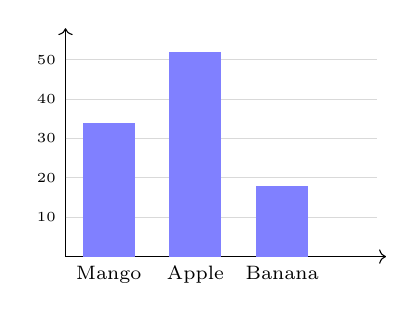
\begin{tikzpicture}[x=0.55cm,y=0.05cm]
  \draw[->] (0,0) -- (7.4,0); \draw[->] (0,0) -- (0,58);
  \foreach \y in {10,20,30,40,50} {\draw[gray!30] (0,\y) -- (7.2,\y);
    \node[left,font=\tiny] at (0,\y) {\y};}
  \foreach \x/\h/\n in {1/34/Mango,3/52/Apple,5/18/Banana} {
    \fill[blue!50] (\x-0.6,0) rectangle (\x+0.6,\h);
    \node[below,font=\scriptsize] at (\x,0) {\n};}
\end{tikzpicture}
\column{0.56\textwidth}
A \textbf{vision-language model (VLM)} takes an image and a question and writes
an answer. We study two open 7B models: \textbf{Qwen2.5-VL} and \textbf{LLaVA-NeXT}.
\vspace{0.6em}

\textbf{Q:} ``What is the value of Mango?''\\
Right answer: 34
\vspace{0.6em}

\textbf{Q:} ``What is the value of Guava?''\\
Right answer: \emph{there is no Guava bar}
\end{columns}
\end{frame}

\begin{frame}{Two different ways to be wrong}
\begin{columns}[T]
\column{0.48\textwidth}
\textbf{Misread} (``structural'')
\begin{itemize}
\item ``Mango?'' $\to$ \alert{30}
\item The answer \emph{was} on the chart; the model read it badly (rounded to a
gridline, took the next bar)
\item Fix: \textbf{look again}, more carefully
\end{itemize}
\column{0.48\textwidth}
\textbf{Fabrication}
\begin{itemize}
\item ``Guava?'' $\to$ \alert{40}
\item The model states something the chart does \emph{not} contain
\item Looking again cannot help. Fix: \textbf{don't answer}
\end{itemize}
\end{columns}
\vspace{1em}
Today's reliability tools give one ``trust / don't trust'' score. They cannot
tell these apart, so they cannot pick the right fix.
\end{frame}

\begin{frame}{Our question}
\begin{center}
\Large Before the model answers, can we tell from its \hl{internal state}\\
whether it is about to be wrong, and \hl{in which way}?
\end{center}
\vspace{1em}
\textbf{Hypothesis (type separability).} The internal state before a misread
differs from the state before a fabrication, because one is a perception error
and the other is an answer not grounded in the image.
\vspace{0.6em}

And if so: does the \textbf{type} decide which fix works?
\end{frame}

% ===========================================================================
\section{Three tools we use}

\begin{frame}{Tool 1: the hidden state}
\centering
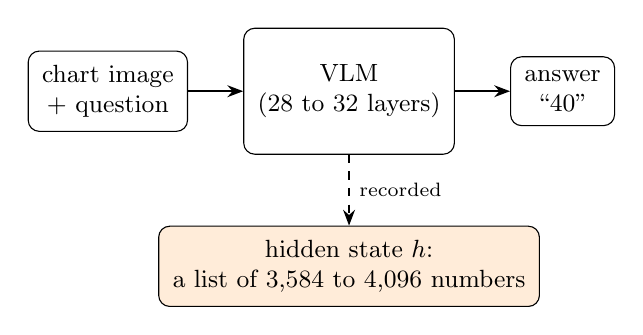
\begin{tikzpicture}[node distance=7mm]
  \node[box] (in) {chart image\\+ question};
  \node[box, right=of in, minimum height=1.6cm] (m) {VLM\\(28 to 32 layers)};
  \node[box, right=of m] (out) {answer\\``40''};
  \node[box, below=9mm of m, fill=orange!15] (h) {hidden state $h$:\\a list of 3,584 to 4,096 numbers};
  \draw[arr] (in) -- (m); \draw[arr] (m) -- (out);
  \draw[arr, dashed] (m) -- node[right,font=\scriptsize] {recorded} (h);
\end{tikzpicture}
\vspace{0.8em}
\raggedright
\begin{itemize}\small
\item Inside, the model turns its input into long vectors of numbers, layer by layer
\item We record the vector at the \textbf{last word of the question}, the moment
just before it writes its first answer word, at every layer
\item Recorded in the same run that produced the answer, so it belongs to exactly that answer
\end{itemize}
\end{frame}

\begin{frame}{Tool 2: a probe}
\begin{columns}[c]
\column{0.48\textwidth}
\centering
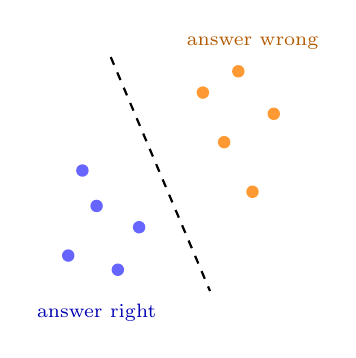
\begin{tikzpicture}[scale=0.9]
  \foreach \x/\y in {0.4/0.6,0.8/1.3,1.1/0.4,0.6/1.8,1.4/1.0}
    \fill[blue!60] (\x,\y) circle (2.5pt);
  \foreach \x/\y in {2.6/2.2,3.0/1.5,2.3/2.9,3.3/2.6,2.8/3.2}
    \fill[orange!80] (\x,\y) circle (2.5pt);
  \draw[thick, dashed] (1.0,3.4) -- (2.4,0.1);
  \node[font=\scriptsize, blue!70!black] at (0.8,-0.2) {answer right};
  \node[font=\scriptsize, orange!70!black] at (3.0,3.6) {answer wrong};
\end{tikzpicture}
\column{0.5\textwidth}
\begin{itemize}
\item A \textbf{probe} is a simple classifier (logistic regression) trained on
hidden states to predict a label, e.g.\ ``will this answer be wrong?''
\item It can only draw a straight line through the space
\item If it succeeds on charts it never saw, the information is plainly
\emph{written in} the model's state
\end{itemize}
\end{columns}
\end{frame}

\begin{frame}{Tool 3: how we score a probe, and why we need baselines}
\textbf{AUROC}: pick one example of each class at random; AUROC is the chance the
probe scores the right one higher.
\begin{center}
0.5 = coin flip \qquad 0.8 = useful \qquad 1.0 = perfect
\end{center}
\vspace{0.4em}
\textbf{Baselines.} A probe can ``succeed'' by reading something trivial, such as
how long the question is. So every probe is compared with:
\begin{itemize}\small
\item the same classifier on \textbf{surface features} only (question type and
length, image size, numeric answer), with no access to the model
\item the probe after those features are \textbf{removed} from the hidden state
\item probes trained \textbf{within one question type}
\end{itemize}
Every number has a 95\% confidence interval, and no chart is in both training and test.
\end{frame}

% ===========================================================================
\section{Part 1: real charts (ChartQA)}

\begin{frame}{What errors do models actually make on real charts?}
\begin{columns}[c]
\column{0.45\textwidth}
\small
\begin{tabular}{lrr}
\toprule
Error label & Qwen & LLaVA \\
\midrule
Misread & 71 & 583 \\
Arithmetic slip & 93 & 435 \\
Not actually wrong & 112 & 69 \\
Unclear & 40 & 74 \\
Fabrication & \hl{1} & \hl{17} \\
\midrule
All errors & 317 & 1,178 \\
\bottomrule
\end{tabular}
\column{0.53\textwidth}
\begin{itemize}\small
\item 2,500 ChartQA questions: Qwen 87\% right, LLaVA 53\%
\item We labelled every wrong answer (LLM annotator, written rubric)
\item \textbf{Fabrication almost never happens} on real charts: questions are
about things the chart shows
\item 35\% of Qwen's ``errors'' are actually right (format, wrong gold)
\item Human check: two of us labelled 200 errors; after settling disagreements,
humans and LLM agree at $\kappa=0.61$
\end{itemize}
\end{columns}
\end{frame}

\begin{frame}{Result 1: we can predict a wrong answer before it is written}
\centering
\begin{tabular}{lccc}
\toprule
AUROC (wrong vs.\ right) & Probe & Surface features only & Features removed \\
\midrule
Qwen & \hl{0.88} & 0.72 & 0.80 \\
LLaVA & \hl{0.80} & 0.61 & 0.78 \\
\bottomrule
\end{tabular}
\vspace{1em}
\raggedright
\begin{itemize}
\item Far above what the question's surface reveals, and most of it survives
removing those features
\item The signal sits in the question-side state in the last third of the
network; the image part alone stays near the surface baseline
\item Stable across five different train/test splits ($\pm$0.02)
\end{itemize}
\end{frame}

\begin{frame}{Result 2: misreads and arithmetic slips look different inside}
\centering
\begin{tabular}{lcc}
\toprule
AUROC & Qwen & LLaVA \\
\midrule
Misread vs.\ correct & 0.89 & 0.81 \\
Arithmetic slip vs.\ correct & 0.90 & 0.95 \\
\hl{Misread vs.\ arithmetic slip} & \hl{0.90} & \hl{0.96} \\
\bottomrule
\end{tabular}
\vspace{1em}
\raggedright
\begin{itemize}
\item Worry: arithmetic slips only happen on ``what is the difference\dots''
questions, so a probe might just spot the wording
\item Check: retrain using only arithmetic questions (0.85 and 0.84), or only
reading questions (0.91 and 0.81). The signal survives
\item On real charts, the two error types models actually make are separable
\end{itemize}
\end{frame}

% ===========================================================================
\section{Part 2: making fabrication happen}

\begin{frame}{Synthetic charts: ask about something that is not there}
We drew 900 bar charts and asked each the same question twice, \textbf{in
identical words}: once about a bar that is shown, once about one that is not.
\vspace{0.6em}
\begin{itemize}
\item Pilot 1: ``What is the value of Mango?'' vs.\ ``\dots of \alert{Guava}?''
\item Pilot 2: lookalike names (Dublin shown, ask \alert{Dubai}); also ``Which is
larger?'' and ``Which bar is next to\dots?''
\item Pilot 3: years 2014 to 2019 shown, ask about \alert{2021}
\end{itemize}
\vspace{0.6em}
Identical wording matters: the question text alone cannot tell which case it
is, so a probe cannot cheat by reading the words.
\end{frame}

\begin{frame}{The models almost never say ``it's not there''}
\centering
\begin{tabular}{lcc}
\toprule
Asked for a missing bar's value (600 questions) & Qwen & LLaVA \\
\midrule
Says it is not shown & \hl{15} & \hl{0} \\
Says ``0'' & 494 & 232 \\
Makes up a number & 91 & 368 \\
\bottomrule
\end{tabular}
\vspace{1em}
\raggedright
\begin{itemize}
\item Qwen mostly says ``0''; when it invents, it usually copies the lookalike bar
(asked Dubai, reports Dublin)
\item LLaVA invents a number for most missing bars
\end{itemize}
\end{frame}

\begin{frame}{\dots but inside, they know the bar is missing}
\centering
\begin{tabular}{lcc}
\toprule
AUROC, missing vs.\ shown name & Qwen & LLaVA \\
\midrule
Probe on hidden state & \hl{0.99 to 1.00} & \hl{0.96 to 1.00} \\
Classifier on the question text only & 0.49 to 0.52 & 0.49 to 0.52 \\
Probe on the image part only & 0.50 & 0.50 \\
\bottomrule
\end{tabular}
\vspace{1em}
\raggedright
\begin{itemize}
\item The models register that the asked bar is missing, \textbf{then answer anyway}
\item The controls are at chance: it is neither the words nor the image alone,
but the model combining the two
\item Qwen knows by layer 2 of 28; LLaVA by about layer 9 of 32
\end{itemize}
\end{frame}

\begin{frame}{Is it really about ``missing'', or about ``can't be answered''?}
Pilot 3: the chart shows 2014 to 2019; we ask about \alert{2021}. Nothing is
``missing'', the question just cannot be answered from the chart.
\vspace{0.6em}
\begin{columns}[T]
\column{0.5\textwidth}
\small
\begin{tabular}{lcc}
\toprule
Answer to 2021 & Qwen & LLaVA \\
\midrule
Says not shown & \hl{102} & 0 \\
``0'' & 76 & 19 \\
Makes up a number & 105 & 281 \\
\bottomrule
\end{tabular}
\column{0.48\textwidth}
\begin{itemize}\small
\item The probe trained on missing \emph{names} also flags out-of-range
\emph{years}: \hl{1.00} (Qwen), \hl{0.91} (LLaVA)
\item It fires whether Qwen then refuses or invents: it tracks ``the chart
can't answer this'', not what the model will say
\end{itemize}
\end{columns}
\end{frame}

\begin{frame}{Misread vs.\ fabrication: does each probe stick to its own type?}
\centering
\begin{tabular}{lcccc}
\toprule
 & \multicolumn{2}{c}{Qwen} & \multicolumn{2}{c}{LLaVA} \\
Scored on $\to$ & misreads & fabrications & misreads & fabrications \\
\midrule
Misread probe & \hl{0.89} & 0.59 & \hl{0.78} & 0.88 \\
Fabrication probe & 0.58 & \hl{1.00} & 0.68 & \hl{0.99} \\
\bottomrule
\end{tabular}
\vspace{0.8em}
\raggedright
\begin{itemize}\small
\item \textbf{Qwen:} each probe is strong on its own type, weak on the other:
separable, as hypothesised
\item \textbf{LLaVA:} the misread probe fires even more on fabrications: one
general ``not grounded'' signal
\item \textbf{Caveat:} on synthetic charts, whether a reading counts as a misread
depends mostly on where the value sits between gridlines; that chart property
alone predicts misreads as well as the probes (0.92 and 0.86)
\end{itemize}
\end{frame}

% ===========================================================================
\section{Part 3: does the type decide the fix?}

\begin{frame}{Four ways to make the model look again}
\begin{columns}[c]
\column{0.5\textwidth}
\begin{itemize}\small
\item \textbf{Re-ask}: same question again (a second try)
\item \textbf{Upsample}: the whole chart, enlarged
\item \textbf{Crop}: only the asked bar and its axis, enlarged
\item \textbf{Verify}: ``first name the part of the chart that supports your
answer''
\end{itemize}
\column{0.48\textwidth}
\textbf{Prediction, written down before running} (pre-registered): cropping should
rescue misreads more than fabrications, since for a fabrication there is nothing
to look at.
\vspace{0.6em}

Applied to every wrong answer on the synthetic charts (Qwen 631, LLaVA 1,015).
\end{columns}
\end{frame}

\begin{frame}{Result: the prediction holds}
\centering
\small
\begin{tabular}{lcccc}
\toprule
Fraction fixed & Re-ask & Upsample & Crop & Verify \\
\midrule
\multicolumn{5}{l}{\textit{Qwen}} \\
Misread & 0.11 & 0.13 & \hl{0.26} & 0.09 \\
Made-up number & 0.00 & 0.00 & 0.00 & \hl{0.14} \\
``0'' & 0.02 & 0.02 & 0.02 & \hl{0.69} \\
\multicolumn{5}{l}{\textit{LLaVA}} \\
Misread & 0.03 & 0.01 & \hl{0.15} & 0.03 \\
Made-up number & 0.00 & 0.00 & 0.00 & 0.00 \\
\bottomrule
\end{tabular}
\vspace{0.6em}
\raggedright
\begin{itemize}\small
\item Crop helps misreads, never fabrications, in both models (pre-registered
test passes: +0.26 and +0.15, both intervals above zero)
\item For Qwen the best fix differs by type: crop for misreads, verify for
missing bars (it makes Qwen say ``not shown'')
\item Nothing we tried fixes LLaVA's missing-bar answers: only abstaining works
\end{itemize}
\end{frame}

\begin{frame}{Putting it together: a type-aware controller}
\begin{columns}[c]
\column{0.5\textwidth}
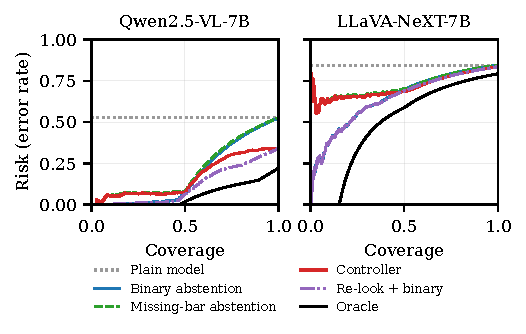
\includegraphics[width=\textwidth]{figures/e5_risk_coverage.pdf}
\column{0.48\textwidth}
\small
\textbf{Controller}: if the missing-bar probe fires, abstain; if the misread
probe fires, look again with the best fix.
\vspace{0.4em}

\textbf{Risk-coverage}: answer only the questions you are most confident about;
plot the error rate against the fraction answered. Lower is better.
\begin{itemize}
\item Re-looking lowers error in both models
\item The controller beats plain ``abstain when unsure'' only for Qwen, mostly by
turning ``0'' into ``not shown''
\item A perfect-knowledge oracle is still far better: room to improve
\end{itemize}
\end{columns}
\end{frame}

% ===========================================================================
\section{Conclusions}

\begin{frame}{What we learned}
\begin{enumerate}
\item A model's internal state predicts that an answer will be wrong
\textbf{before} it is written, beyond the question's surface
\item On real charts the errors are misreads and arithmetic slips, and they look
\textbf{different} inside the model
\item Models \textbf{know} when a chart cannot answer the question, and answer
anyway. This ``unanswerable'' signal is the most useful one for deciding when to
abstain
\item The type does change the best fix: cropping rescues misreads, not
fabrications, as we predicted in advance
\end{enumerate}
\end{frame}

\begin{frame}{Limitations}
\begin{itemize}
\item Fabrication is rare on real charts, so the misread vs.\ fabrication
comparison rests on synthetic bar charts
\item On synthetic charts, misreads largely reflect chart geometry, and those
probes do not carry over to real charts
\item Error labels come from an LLM annotator; two humans agreed with each other
only moderately ($\kappa=0.42$)
\item Repairs and the controller are tested on synthetic charts only
\item Probes show what is encoded, not that the model uses it
\end{itemize}
\end{frame}

\begin{frame}[standout]
Thank you\\[0.6em]
{\normalsize Code and results: github.com/the-neemon/type-aware-vlm-failures}
\end{frame}

\end{document}
